% Contribución de la Persona 2 para integrar en el artículo conjunto.
% Requiere graphicx, booktabs, tabularx, array, float y placeins en el preámbulo.

\section{Estado del arte}
\label{sec:estado-arte-p2}

El problema de planificación universitaria basada en planes de estudio (Curriculum-Based Course Timetabling, CB-CTT) consiste en asignar cada clase a un periodo y un aula. El horario debe respetar las restricciones obligatorias y reducir las penalizaciones asociadas a las preferencias. Incluso después de obtener una solución factible, el número de alternativas posibles sigue siendo elevado, por lo que buena parte de la literatura recurre a metaheurísticas \cite{ceschia2023educational}.

\subsection{Metaheurísticas}

Los primeros trabajos sobre CB-CTT combinaron movimientos de reasignación e intercambio con Hill Climbing y búsqueda tabú. En la Segunda Competición Internacional de Horarios de 2007 (Second International Timetabling Competition, ITC-2007), el método de Müller obtuvo el mejor resultado en la modalidad dedicada a este problema. Su propuesta coordina cinco tipos de movimiento con Hill Climbing, Gran Diluvio (Great Deluge) y enfriamiento simulado \cite{muller2009itc}. Hill Climbing conserva los cambios que mejoran el horario, Great Deluge utiliza un umbral de aceptación que varía durante la búsqueda y el enfriamiento simulado permite aceptar algunos empeoramientos.

En un problema de minimización, el enfriamiento simulado acepta siempre una mejora y admite un empeoramiento de magnitud $\Delta$ con probabilidad $\exp(-\Delta/T)$. La temperatura $T$ disminuye durante la ejecución. Al principio se aceptan más cambios desfavorables, lo que permite salir de un horario que parece bueno solo dentro de su entorno inmediato. Conforme baja la temperatura, esos cambios se vuelven menos probables y la búsqueda se concentra en reducir el coste. La Fig.~\ref{fig:sa-flow} resume este ciclo. En el problema estudiado, cada solución nueva es un horario vecino y la decisión de aceptarlo depende del cambio en la penalización y de la temperatura.

\begin{figure}[H]
  \centering
  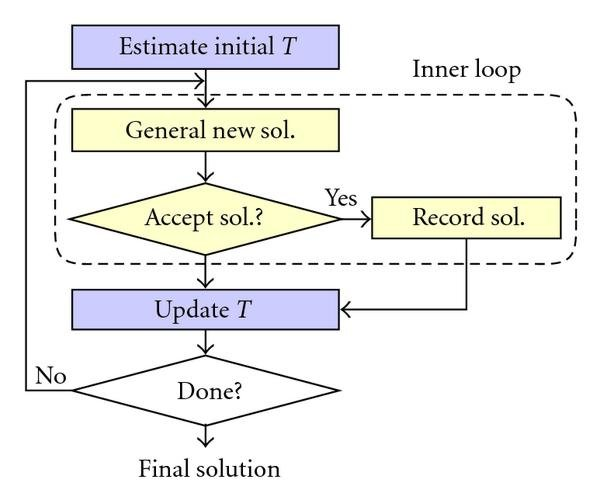
\includegraphics[width=0.76\columnwidth]{figures/paper/simulated_annealing_flow.png}
  \caption{Ciclo general del enfriamiento simulado. Para CB-CTT, la nueva solución corresponde a un horario vecino y la temperatura regula la aceptación de los cambios que aumentan su penalización. Reproducido de la Fig.~1 de Ababei \cite{ababei2009fpga}.}
  \label{fig:sa-flow}
\end{figure}

Bellio et al. aplicaron este esquema a CB-CTT y mostraron que la temperatura inicial influye de forma directa en la calidad final \cite{bellio2016feature}. Song et al. lo ampliaron con varios tipos de movimiento y ajustaron la frecuencia con la que se seleccionaba cada uno \cite{song2021competition}. Cuando existen varios movimientos, la búsqueda también debe decidir cuál aplicar en cada momento. La búsqueda de vecindario variable (Variable Neighborhood Search, VNS) cambia de vecindario cuando el actual deja de producir mejoras. El descenso por vecindarios variables (Variable Neighborhood Descent, VND) sigue una secuencia fijada de búsquedas locales. Las hiperheurísticas llevan esta decisión a un nivel superior y seleccionan el movimiento de bajo nivel que se aplicará a continuación.

Otros métodos amplían la búsqueda manteniendo varios horarios a la vez. Abdullah et al. combinan una población de soluciones con un mecanismo inspirado en electromagnetismo y Great Deluge \cite{abdullah2012hybrid}. La incorporación de componentes con funciones diferentes conduce a los métodos híbridos, cuyo uso creciente en planificación universitaria recoge la revisión de Abdipoor et al. \cite{abdipoor2023meta}.

\subsection{Métodos híbridos}

Los métodos híbridos combinan técnicas que intervienen en momentos distintos de la búsqueda. Un algoritmo memético, por ejemplo, genera varios horarios y aplica una búsqueda local para mejorar algunos de ellos. En una matheurística, el algoritmo retira temporalmente un conjunto de clases del horario y formula su recolocación como un problema matemático. Kiefer et al. siguen este segundo enfoque mediante una búsqueda adaptativa de gran vecindario (Adaptive Large Neighborhood Search, ALNS) \cite{kiefer2017adaptive}. La parte adaptativa elige qué clases conviene retirar según el rendimiento reciente de cada regla y el modelo exacto vuelve a asignarlas sin alterar el resto del horario. Así se exploran cambios amplios sin perder el control sobre las restricciones.

Otra posibilidad consiste en combinar una población de horarios con una regla de aceptación propia de la búsqueda local. Abdullah et al. asignan a cada horario una fuerza calculada a partir de su penalización y emplean esa información para dirigir Great Deluge \cite{abdullah2012hybrid}. La Fig.~\ref{fig:hybrid} muestra el mecanismo sobre horarios concretos. Las soluciones con menor penalización atraen la búsqueda, las peores la alejan y la combinación produce un nuevo horario.

\begin{figure}[H]
  \centering
  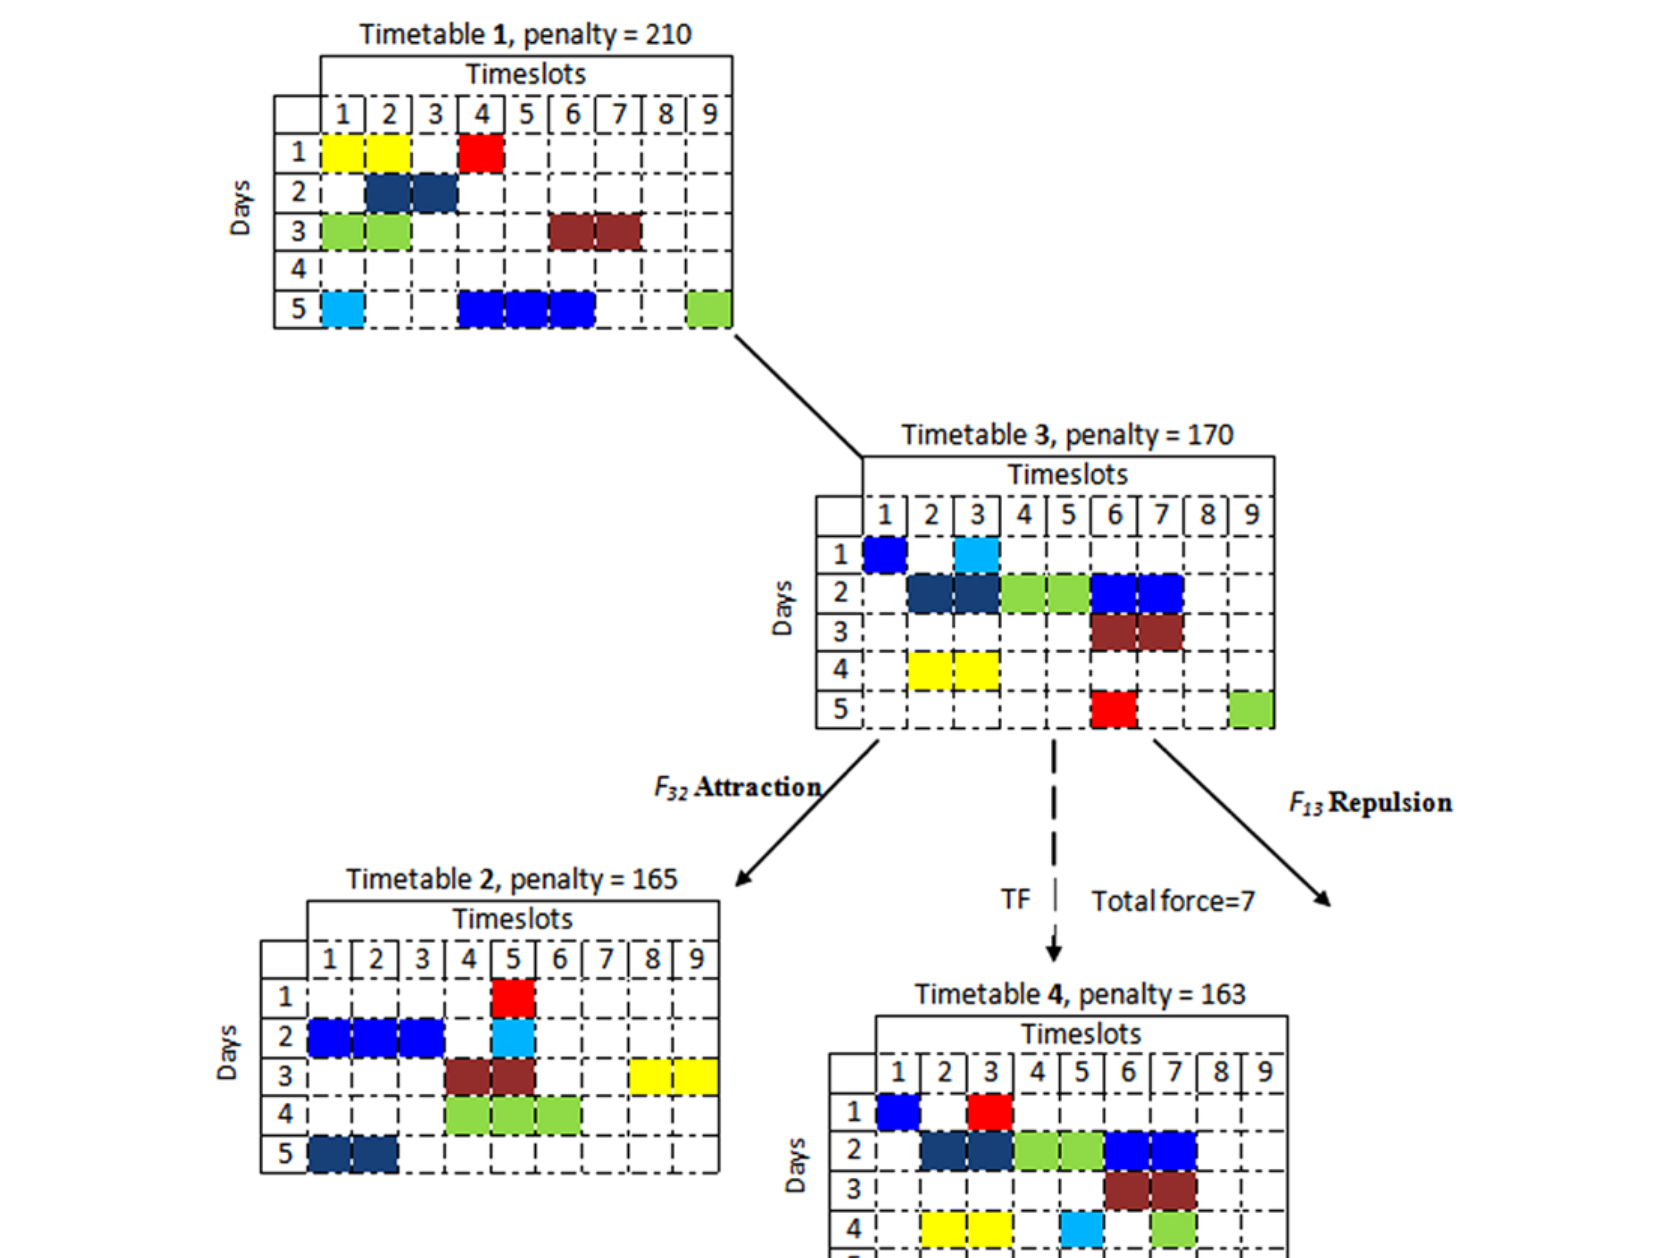
\includegraphics[width=0.98\columnwidth]{figures/paper/hybrid_attract_repel.png}
  \caption{Ejemplo del componente de atracción y repulsión del método híbrido de Abdullah et al. Los horarios con penalizaciones 210 y 165 modifican la búsqueda iniciada desde el horario con penalización 170, que conduce a una nueva solución con penalización 163. Reproducido de la Fig.~2 de Abdullah et al. \cite{abdullah2012hybrid}.}
  \label{fig:hybrid}
\end{figure}

\subsection{Nuevas líneas de investigación}

Una línea reciente estudia cómo adaptar el algoritmo a cada instancia antes de comenzar la búsqueda. De Coster et al. describen cada problema mediante 256 características y entrenan selectores que recomiendan el algoritmo más apropiado para cada región del espacio de instancias \cite{decoster2022algorithm}. Este planteamiento desplaza la pregunta desde qué método es mejor en promedio hacia qué método conviene utilizar ante una estructura concreta de conflictos, aulas y disponibilidad.

El paso siguiente sería trasladar esa adaptación a la propia búsqueda. En lugar de mantener fijas las probabilidades de los movimientos, el algoritmo podría actualizarlas según su rendimiento reciente. También queda por estudiar si un selector entrenado con los horarios de una universidad conserva su utilidad cuando cambian las restricciones y la estructura de los planes de estudio.

En el método que se reproduce, Hill Climbing obtiene un horario factible y el enfriamiento simulado decide si acepta cada modificación. LectureKick es la regla que construye esa modificación respetando las restricciones del horario. Por eso el vecindario conecta la estrategia de aceptación con la estructura concreta de CB-CTT.

\section{El vecindario LectureKick}
\label{sec:lecturekick}

LectureKick es la regla de vecindario con la que el algoritmo genera el siguiente horario. Ceschia et al. la aplican después de una inicialización mediante Hill Climbing y dentro de una fase de enfriamiento simulado \cite{ceschia2026revisiting}. La regla reubica una o dos clases sin incumplir las restricciones obligatorias. Antes de aplicarla, el programa construye un horario factible y calcula las cuatro penalizaciones blandas del problema.

Cada clase ocupa un hueco definido por un periodo y un aula. En la notación de la Fig.~\ref{fig:lecturekick}, $l_i$ identifica una clase, $c_i$ indica el curso al que pertenece esa clase y $s_i$ representa un hueco del horario. Por ejemplo, $l_2\!:\!c_2$ significa que la segunda clase pertenece al curso $c_2$. LectureKick parte de $l_1$ situada en $s_1$ y propone trasladarla a $s_2$. Si el destino está libre, basta con mover $l_1$. Cuando $s_2$ contiene otra clase $l_2$, LectureMove solo permite enviarla al hueco liberado $s_1$. LectureKick añade la posibilidad de colocar $l_2$ en cualquier hueco libre $s_3$. De este modo puede alcanzar horarios que no están disponibles mediante un intercambio directo.

\begin{figure}[H]
  \centering
  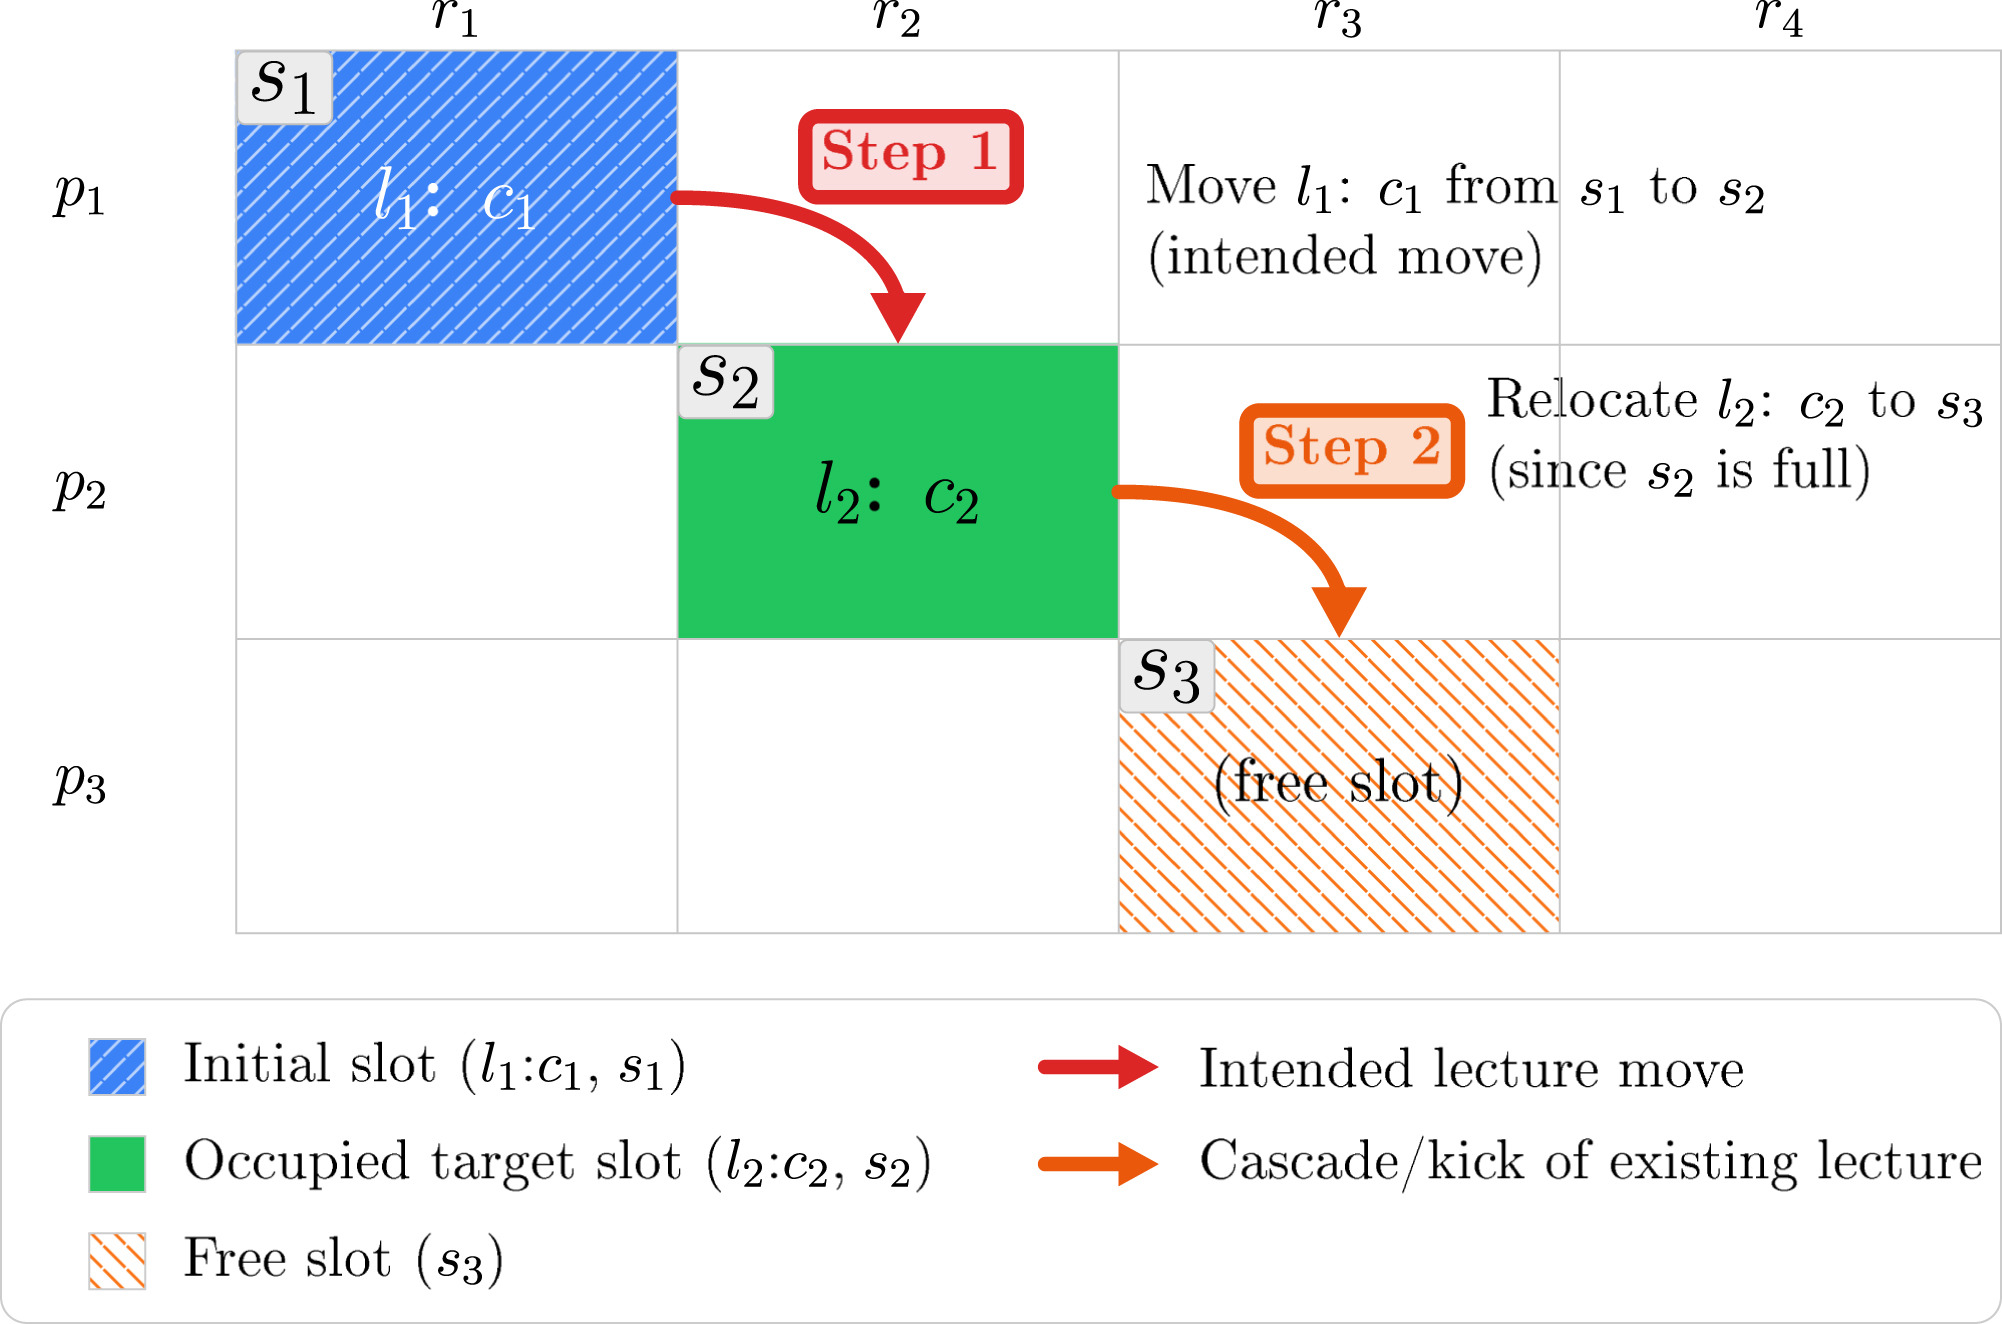
\includegraphics[width=\columnwidth]{figures/paper/gr1_lrg.jpg}
  \caption{Movimiento LectureKick. El símbolo $l_i$ identifica una clase, $c_i$ su curso y $s_i$ un hueco formado por periodo y aula. La clase $l_1$ pasa de $s_1$ a $s_2$ y, si el destino está ocupado, $l_2$ puede reubicarse en $s_3$. Reproducido de la Fig.~1 de Ceschia et al. \cite{ceschia2026revisiting}.}
  \label{fig:lecturekick}
\end{figure}

Los destinos deben ser distintos, los periodos deben estar disponibles y las clases implicadas no pueden presentar conflictos. Cuando se utiliza $s_3$, ese hueco debe permanecer libre. Estas condiciones hacen que la regla trabaje únicamente con horarios factibles.

La elección de los movimientos tampoco es uniforme. Un sesgo favorece las clases que todavía no alcanzan el mínimo de días y otro da prioridad a los cursos con riesgo de generar clases aisladas. El algoritmo también prefiere aulas ya utilizadas por el mismo curso y aulas con capacidad suficiente. Un último sesgo aumenta la frecuencia de los intercambios propios de LectureMove. La Fig.~\ref{fig:sesgos} reproduce los ejemplos con los que los autores explican estas seis decisiones.

\begin{figure}[!t]
\centering
\begin{minipage}{0.48\columnwidth}\centering
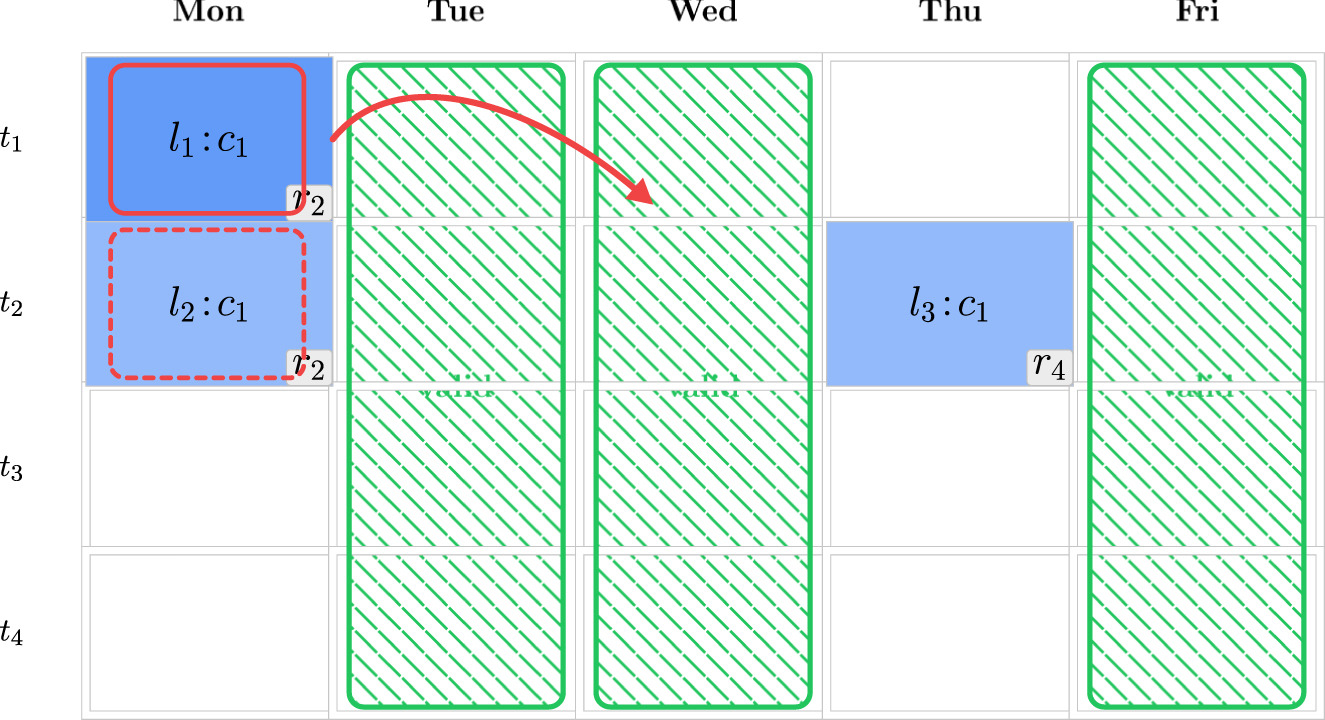
\includegraphics[width=\linewidth]{figures/paper/gr2a_lrg.jpg}\\[-1mm]
\scriptsize (a) Días mínimos
\end{minipage}\hfill
\begin{minipage}{0.48\columnwidth}\centering
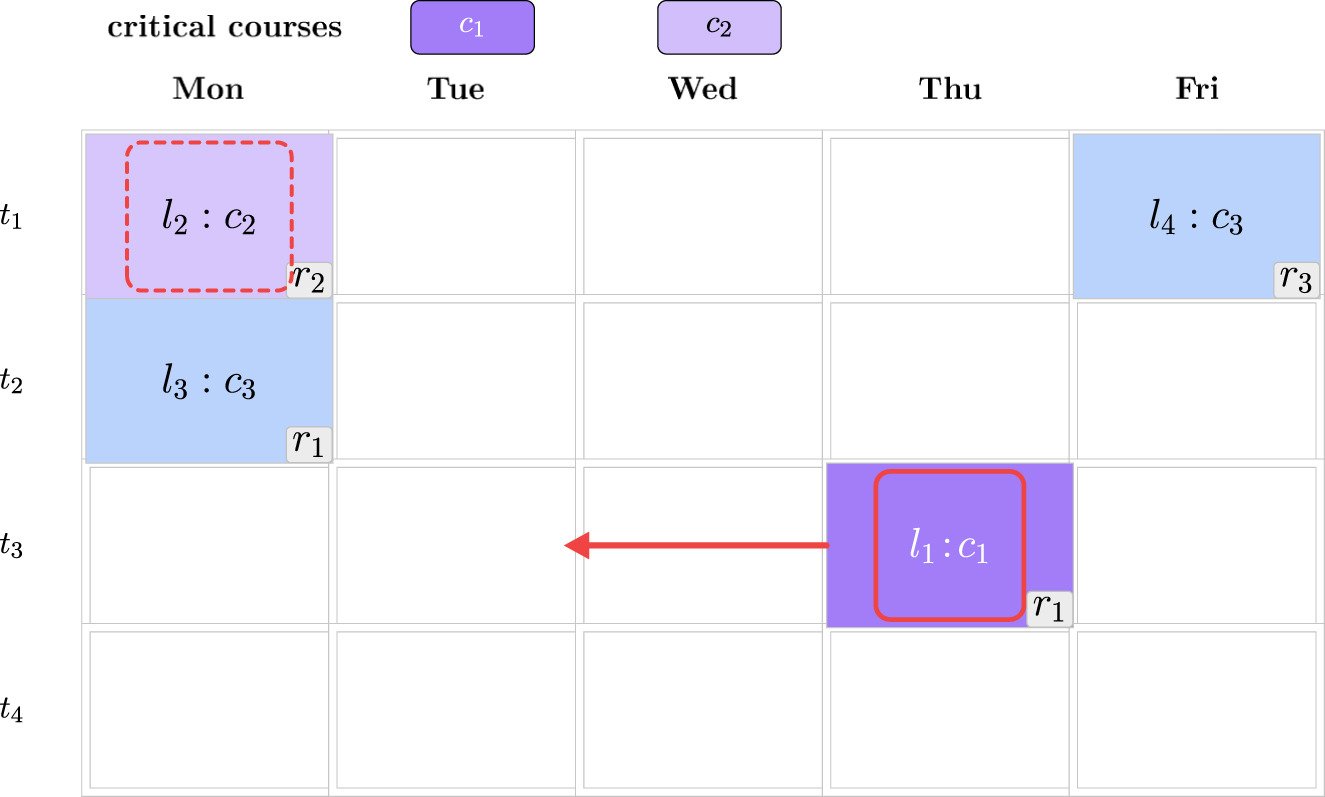
\includegraphics[width=\linewidth]{figures/paper/gr2b_lrg.jpg}\\[-1mm]
\scriptsize (b) Clases aisladas
\end{minipage}

\vspace{1mm}
\begin{minipage}{0.48\columnwidth}\centering
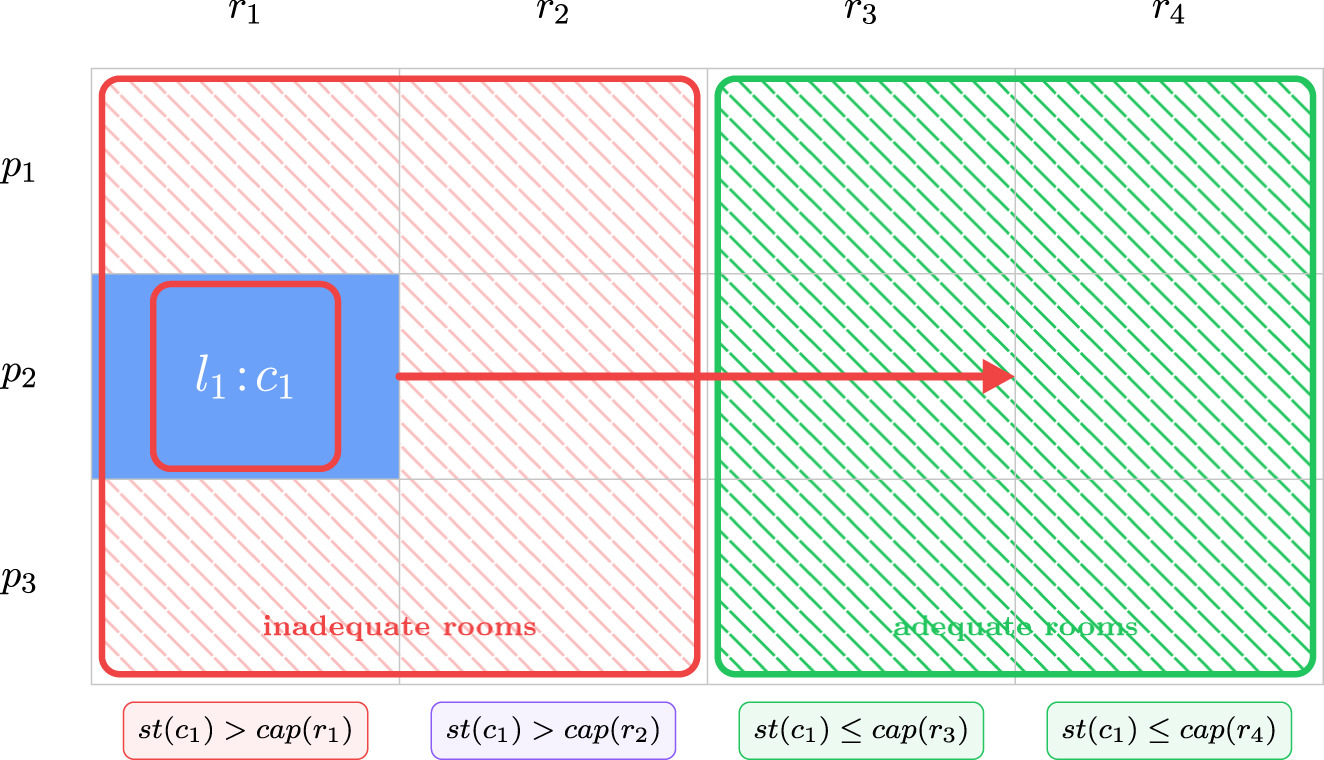
\includegraphics[width=\linewidth]{figures/paper/gr2c_lrg.jpg}\\[-1mm]
\scriptsize (c) Capacidad del aula
\end{minipage}\hfill
\begin{minipage}{0.48\columnwidth}\centering
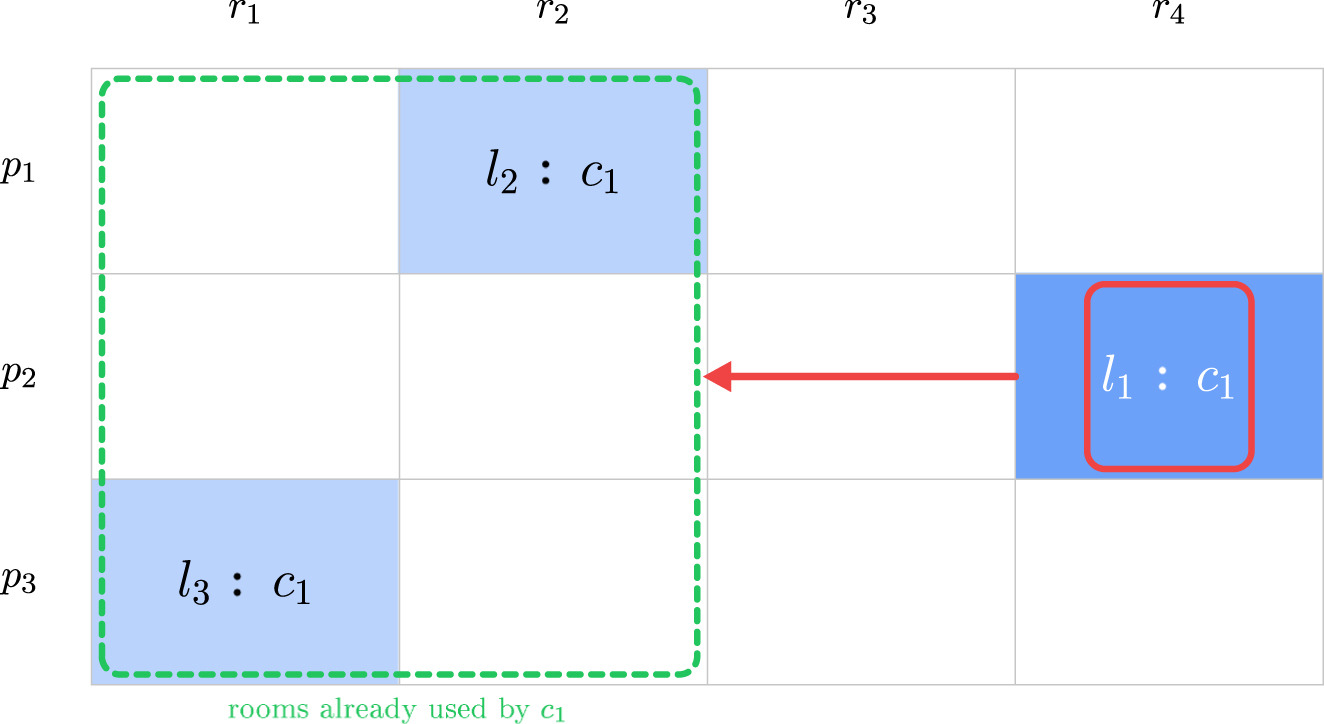
\includegraphics[width=\linewidth]{figures/paper/gr2d_lrg.jpg}\\[-1mm]
\scriptsize (d) Estabilidad del aula
\end{minipage}\hfill

\vspace{1mm}
\begin{minipage}{0.48\columnwidth}\centering
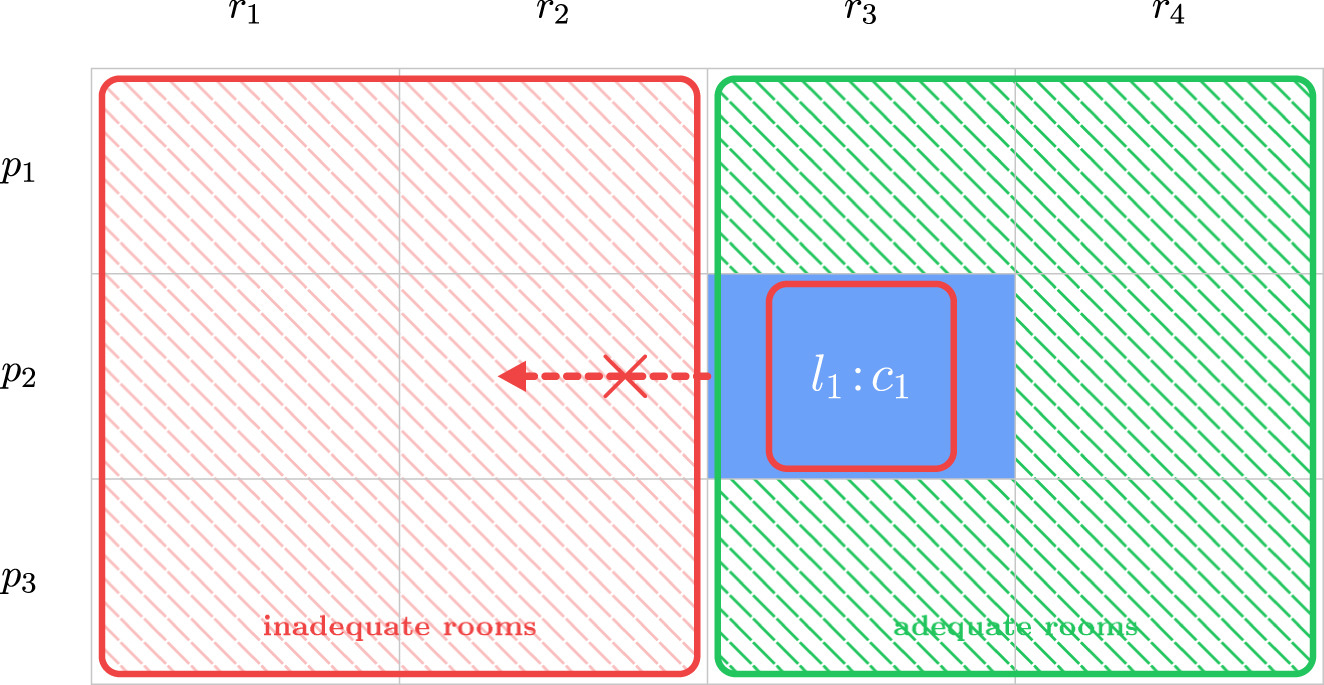
\includegraphics[width=\linewidth]{figures/paper/gr2e_lrg.jpg}\\[-1mm]
\scriptsize (e) Prevención de capacidad
\end{minipage}\hfill
\begin{minipage}{0.48\columnwidth}\centering
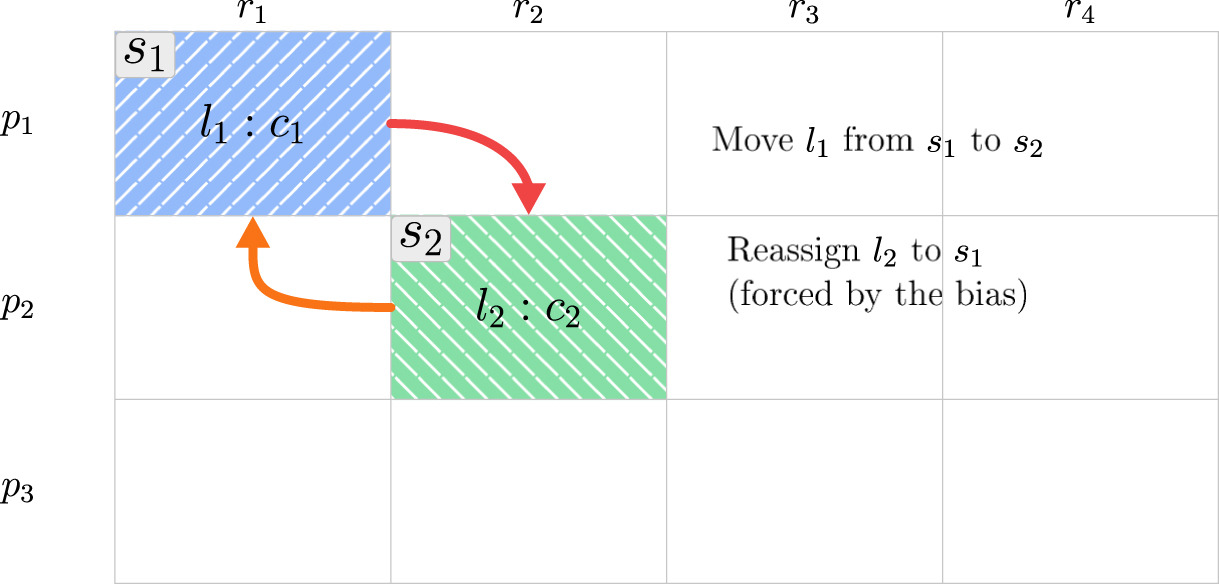
\includegraphics[width=\linewidth]{figures/paper/gr2f_lrg.jpg}\\[-1mm]
\scriptsize (f) Preferencia de intercambio
\end{minipage}
\caption{Ejemplos de los seis sesgos de selección empleados con LectureKick. Los cuatro primeros actúan sobre penalizaciones blandas. Los otros dos evitan una penalización de capacidad y favorecen los intercambios. Reproducido de la Fig.~2 de Ceschia et al. \cite{ceschia2026revisiting}.}
\label{fig:sesgos}
\end{figure}
\FloatBarrier

Ceschia et al. no fijaron estos parámetros manualmente. Antes de los experimentos finales usaron \texttt{irace}. El programa prueba varias combinaciones en un conjunto de instancias y descarta las que funcionan peor. Después repite la comparación con las restantes hasta escoger una configuración. El proceso se aplica a la temperatura, al enfriamiento y a las probabilidades de los seis sesgos \cite{ceschia2026revisiting,lopezibanez2016irace}. Una vez elegidos, esos valores permanecen fijos durante LectureKick.

\section{Metodología de reproducción}
\label{sec:reproduccion}

Se ejecutó el programa publicado por Ceschia et al. con la configuración utilizada en el artículo \cite{ceschia2026revisiting}. El proceso comienza con Hill Climbing para obtener un horario factible y continúa con el enfriamiento simulado, que utiliza LectureKick para generar horarios vecinos.

\subsection{Diseño experimental}

Se seleccionaron las 19 instancias no redundantes de la formulación UD2 de ITC-2007. Se omitió \texttt{comp11} porque su coste objetivo es nulo y \texttt{comp15} porque equivale a \texttt{comp03} bajo esta formulación. Cada instancia se ejecutó tres veces con semillas distintas, lo que dio lugar a 57 ejecuciones. El programa convirtió el límite virtual de 192 segundos en un presupuesto de búsqueda específico para cada instancia.

En cada ejecución, el programa construyó primero un horario y aplicó Hill Climbing hasta alcanzar una solución factible. Después utilizó el enfriamiento simulado con LectureKick hasta agotar el presupuesto asignado. Al finalizar se comprobó que no hubiera violaciones obligatorias y se registraron la penalización final y el tiempo. Con estas comprobaciones se puede verificar la ejecución del método y dejar preparados los datos para el análisis y la comparación posterior de resultados.

Por limitaciones computacionales, la reproducción emplea tres semillas por instancia frente a las 30 del artículo y se ejecuta en un entorno diferente, por lo que permite comprobar el procedimiento y la factibilidad, pero los tiempos solo son orientativos. La Tabla~\ref{tab:entorno} resume las diferencias técnicas \cite{boulesteix2019benchmarking}.

\begin{table}[H]
\caption{Diferencias técnicas entre las ejecuciones}
\label{tab:entorno}
\centering
\scriptsize
\begin{tabular}{@{}lll@{}}
\toprule
Aspecto & Artículo & Reproducción \\
\midrule
CPU & No indicado & i7-9700F (8 núcleos) \\
SO & Ubuntu 24.04 & Windows 10 Pro \\
Compilador & G++ 13.3 & G++ 16.2 / UCRT64 \\
\bottomrule
\end{tabular}
\end{table}
